\section{Analyse de l'existant}

La première version de plate-forme d’\ezb\ a été lancée, puis arrêtée, par une équipe de développeurs, du faite des difficultés en termes de conception et de code. Quand je suis arrivée, la nouvelle version de la conception et de la structure des codes de la plate-forme qui s'est appellée \textbf{\mini\ } \footnote{Le nom \mini\ indiquait la légèreté de la nouvelle structure et contrastait avec l'ancienne version ; son développement avait été réalisé par Ophir LOJKINE, un camarade qui a travaillé sur ce projet pendant quelques mois. }

Afin de découvrir les principes de ces plateformes, pendant le premier moins, j’ai analysé les concepts, choix technologiques et codes de l'\ezb\ et du \mini\ .  

\subsection{Analyse de la conception}
La conception proposée par la plate-forme d’\ezb\ est :
\begin{wrapfigure}{r}{0.25\textwidth}
    \centering
    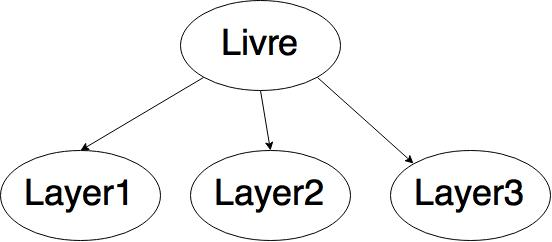
\includegraphics[width=0.25\textwidth]{conception_ezb}
\end{wrapfigure}
\begin{itemize}
    \item un ensemble de layers \footnote{Dans le cadre d'\ezb\ , layer représente la conception de couche où on peux ajouter des citations et résumés} fondé sur un livre
    \item chaque layer devait contenir une liste de citations du texte original et de résumés
\end{itemize}
Avec cette conception, on ne peut pas créer une structure multi-échelles qui permet d'une création de sous-layer d'un layer, ce qui est intéressant pour faire des commentaires, etc.

La conception était améliorée par Ophir qui a proposé une stratégie de création de layers plus adaptable : \textbf{les Couches à thème}. Dans cette version, 

\begin{wrapfigure}{r}{0.4\textwidth}
    \centering
    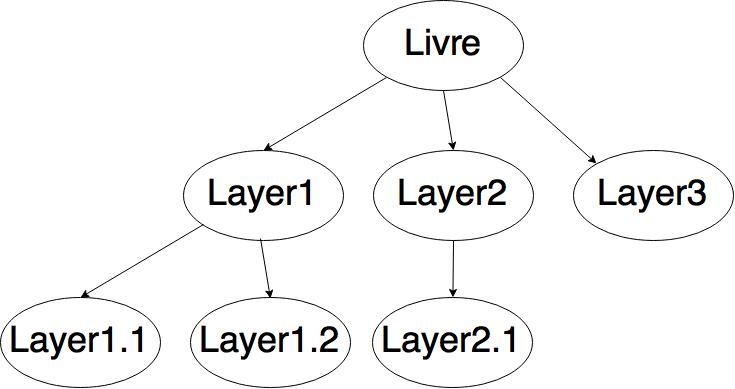
\includegraphics[width=0.4\textwidth]{conception_mini}
\end{wrapfigure}

\begin{itemize}
    \item le livre d'un projet est traité comme un layer
    \item des layers sont fondés sur quelconque layer du projet
    \item chaque layer devait contenir un thème comprenant citation, résumé, traduction, ect
\end{itemize}

\subsection{Analyse des fonctionnelles}
Les changements fonctionnels de \mini\ étaient concentrés sur les parties des gestions de livres et de projets. 
Les parties des gestions d'utilisateurs et de groupes sont bien définies dans \ezb\ , mais pas dans \mini\ .  

\subsubsection{La gestion de livres}
\begin{center}
\begin{tabular}{ |c|c|c| }
\hline
\ezb\ & \mini\ \\ 
\hline
Format ePub                  &  Multi-format \\ 
Gardé comme un fichier .epub &  Gardé dans \db\ en structure \\ 
Non téléchargeable         &  Téléchargeable en multi-format \\
\hline
\end{tabular}
\end{center}

\subsubsection{La gestion de projets}
\begin{center}
\begin{tabular}{ |c|c|c| }
\hline
\ezb\ & \mini\ \\ 
\hline
4 niveaux de finalités à choisir par les utilisateurs \footnotemark & Finalité des paragraphes et des chapitres \\ 
Création de layers du livre & Création de layers à partir d'autres layers \\ 
Citations et résumés & Citation et tous types d'écritures possibles \\
\hline
\end{tabular}
\end{center}
\footnotetext{ Higly Detailed, Fairly Detailed, Fairly Abridged et Highly Abridged } 

\subsubsection{La gestion d'utilisateurs}
Dans \ezb\ , il faut s'inscrire dans le site et tous les utilisateurs sont dans le même niveau de droits qui permet d'accéder à toutes les fonctions de la plate-forme.

\subsubsection{La gestion de groups}
Dans \ezb\ , il y a 3 rôles correspondant aux différents niveaux de droits : pour chaque membre ajouté, on définie un rôle :
\begin{itemize}
    \item \textbf{Owner} qui a tous les droits.
    \item \textbf{Coordinator} qui a le droit d'ajouter des membres.
    \item \textbf{Collaborator} qui n'a pas le droit de gérer le groupe.
\end{itemize}

\subsection{Analyse des choix techonologiques}
\begin{center}
\begin{tabular}{|m{5em}|m{5cm}|m{5cm}|}
\hline
& \ezb\ & \mini\ \\ 
\hline
Langage & Scala & JavaScript \\ 
\hline
Database & NoSQL & SQL \\ 
\hline
\end{tabular}
\end{center}

\begin{figure}[H]
\centering
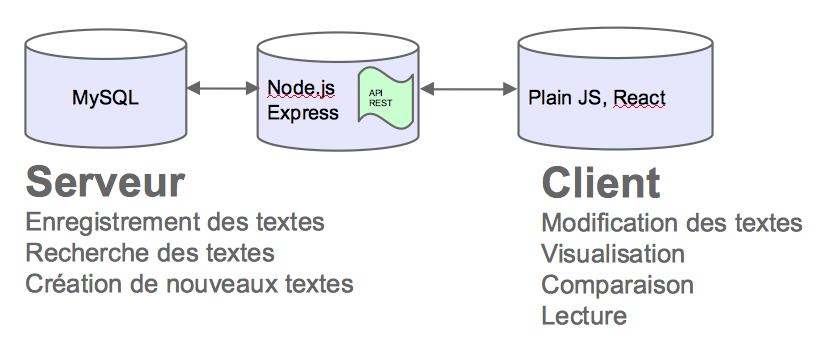
\includegraphics[width=\textwidth]{tech}
\caption{Technologiques choisies}
\end{figure}

Après des discussions avec Ophir, j'ai compris les intérêts de ces nouveaux choix.

En comparaison de \textbf{Scala}, \textbf{JavaScript} est un langage plus davantage utilisé par des développeurs web qui donne à la communauté de développeurs une plus grande possibilité de contribution. 

\textbf{Node.js}, une plateforme logiciel libre en JavaScript orientée vers les applications réseau qui doivent pouvoir monter en charge,  rend possible de faire tourner un serveur web sans avoir besoin d'un logiciel externe comme Apache ou Lighttpd, et permettant de mieux contrôler la façon dont le serveur web fonctionne. Avec une communauté très active dans laquelle beaucoup de modules robustes existent et un système de paquet intégré (NPM), le développement avec Node.js ressemble à un jeu de construction, et permet d'accélérer le développement.

\textbf{Express.js} est choisi comme le framwork parce qu'il s'agit en fait d'un micro-framework pour Node.js et il fournit des outils de base pour aller plus vite dans la création d'applications Node.js. Pour le côté de clients, on a choisi \textbf{React.js}, une bibliothèque orientée Composant. Dans la fonction d'édition, une manière puissante de traiter les changements des text est founie par React.js parce qu'il fonctionne sur le concept d'un \textbf{DOM virtuel}. DOM virtuel fait un diff rapide des changements, tous les lots dans une mise à jour et frappe le DOM réelle tout à la fois. 

Pour une flexibilité plus grande puisque on a besoin d'ancres pour s'assurer que les parties correspondent bien entre un layer et son parent layer, \textbf{SQL} est choisi pour garder des ancres et des contenus de layers. C'est aussi parce que nous avons la pratique de cet outil dans l'école, ce qui simplifie développement. 